\section{Methodik}
% Einleitung
In diesem Abschnitt werden das Design des Experiments, sowie eine kurze Beschreibung der verwendeten Technologien und Daten vorgestellt.
Es wird im Detail erläutert, wie das Experiment aufgebaut ist und welche Ziele damit verfolgt werden.
Die konkrete Auswertung der erhobenen Daten wird im folgenden \autoref{sec:results} vorgestellt.\\

% Datensatz
Für das Experiment liegen die von \textcolor{red}{NAME} bereitgestellten Daten vor.
Es handelt sich dabei um Artikel vom Focus-Magazin\footnote{\url{https://www.focus.de}} zum Thema Elektromobilität.
Diese Artikel wurden durch \textcolor{red}{Soziologen} aufbereitet und in die, im \autoref{subsec:economics-of-conventions} erwähnten, Welten der \ac{EC} eingeteilt.
Der Datensatz besteht aus 26 Artikeln, welche in die Welten Markt, Industrie, \textcolor{red}{TODO} und Grün unterteilt wurden.
Im Datensatz ist die Welt als \textcolor{red}{TODO} benannt, da es in der Literatur unterschiedliche Übersetzungen und Bezeichnungen für die Welten gibt.
Zusätzlich zu der Kategorisierung in eine Welt, enthält der Datensatz die Rechtfertigung bezüglich der Welt.
Diese Rechtfertigung gibt an, ob der Artikel für, gegen oder aus beiden Richtungen bezüglich einer Welt ist.
Dabei bedeutet aus beiden Richtungen nicht, dass der Artikel neutral ist, sondern dass Textabschnitte im Artikel auftauchen, welche für und gegen die Welt sprechen.\\

% Vorstudie
Es wurde ebenfalls eine qualitative Vorstudie durchgeführt, welche die Grundlage für die Masterarbeit bildet.
Diese Vorstudie wurde durch \textcolor{red}{NAME} durchgeführt und \textcolor{red}{TODO: Anhang + cite Studie}.
Zweck dieser Vorstudie war es, neue Darstellungsformen der Artikel-Navigation im Online-Journalismus zu erforschen.
Unter anderem hat sich in dieser Vorstudie herausgestellt, dass die Darstellung als Begriffsverband für fünf von acht Testpersonen als informativ und interessant empfunden wurde.
Allerdings gab es auch zahlreiche Kritikpunkte am Begriffsverband in der Vorstudie.
Der Begriffsverband wies für drei Personen eine hohe Komplexität auf.
Diese sorgt dafür, dass entweder eine lange Einarbeitungszeit nötig ist oder Nutzende abgeschreckt werden.
Ebenfalls ist die Unterteilung in unterschiedliche Rechtfertigungen (positiv, negativ oder beides) bezüglich einer Welt für zwei Personen eher verwirrend als sinnvoll.\\

\subsection{Versuchsaufbau}
Um die Effektivität des Begriffsverbandes in Bezug auf die Auseinandersetzung mit diversen Inhalten zu untersuchen, wurden zwei Prototypen entwickelt.
Der erste Prototyp ähnelt einer klassischen Listenansicht, welche auf einem content-based \ac{RS} basiert.
Der zweite Prototyp ist ein Begriffsverband, welcher auf der vorher genannten Vorstudie aufbaut.
Beide Prototypen wurden mithilfe der Design- und Prototyping-Software Adobe XD von Adobe entwickelt\footnote{\url{https://www.adobe.com/}}.
Adobe XD ermöglicht es, Prototypen ohne Code zu erstellen und diese anschließend mit Testpersonen zu testen.
Die Entscheidung für Adobe XD basiert darauf, dass in der Vorstudie bereits mit dieser Software gearbeitet wurde.
Es bestanden keine Vorerfahrungen mit dieser Software, jedoch mit einer ähnlichen Software namens Figma\footnote{\url{https://www.figma.com/}}.
Die Teilnehmenden dieses Experiments sollen durch beide Prototypen navigieren und anschließend Aufgaben lösen, welche das Verständnis für die jeweiligen Systeme testet.
Im Anschluss an die Aufgaben werden die Teilnehmenden pro Prototyp mithilfe von drei unterschiedlichen Fragebögen zu ihrer Meinung zu den Systemen befragt.\\

Das Experiment soll zeigen, dass der Begriffsverband, in Bezug auf die Auseinandersetzung mit diversen Inhalten, effektiver als eine klassische Listenansicht ist.
Also, dass die Teilnehmenden des Experiments mehr Artikel aus unterschiedlichen Welten der \ac{EC} lesen, wenn sie durch den Begriffsverband navigieren.
Die Testpersonen sollen sich mithilfe der Prototypen zur Elektromobilität informieren.
Dabei werden sie nach fünf gelesenen Artikeln gestoppt und sollen anschließend die erwähnten Aufgaben zum Verständnis der Systeme lösen.
Es wurde sichergestellt, dass jeder Prototyp die gleiche Anzahl an Artikeln und Welten enthält.
Auf diese Weise wird sichergestellt, dass beide Prototypen miteinander vergleichbar sind.\\

Den Testpersonen wurde gesagt, dass sie ihre Gedanken während der Navigation durch die Prototypen laut aussprechen sollen.
Die unterschiedlichen Aussagen der Personen wurden, nach Erklärung des Datenschutzes, aufgezeichnet.
Zur Anonymisierung der Daten wurden die Aufzeichnungen transkribiert und die Namen der Testpersonen durch Pseudonyme ersetzt.
Anschließend wurden alle Aufzeichnungen im Rahmen der Datenschutzerklärung gelöscht.\\

\subsection{Prototyp - Listenansicht}
Der Listenprototyp stellt eine klassische Listenansicht dar.
Bei dieser Listenansicht steht der angeklickte Artikel im Vordergrund und die vom \ac{RS} empfohlenen Artikel werden rechts neben dem angeklickten Artikel in einer Liste dargestellt.
Die Auflistung dieser Artikel erfolgt nach der Relevanz des Artikels für die nutzende Person.
In diesem Fall ist der Parameter, welcher die Relevanz bestimmt, die Ähnlichkeit zum Artikel, welcher gerade gelesen wird.
Die Ähnlichkeit wurde manuell definiert.
Dabei richtet sich Ähnlichkeit danach, welche Welten der \ac{EC} den Artikel zugeordnet wurden.
Dadurch wird ein content-based \ac{RS} simuliert, welches die Artikel bezüglich der Ähnlichkeit ihres Inhalts empfiehlt.\\
\begin{table}
    \centering
    \newcolumntype{I}{>{\centering\arraybackslash}p{10pt}}
    \newcommand{\x}{$\times$}
    \newcommand{\unused}{\cellcolor{gray!60}}
    \resizebox{0.9\textwidth}{!}{
        \begin{minipage}{0.5\linewidth}
            \centering
            \begin{tabular}{|l||I|I|I|I|I|I|I|I|}
                \hline
                   & \multicolumn{2}{c|}{Markt} & \multicolumn{2}{c|}{Industrie} & \multicolumn{2}{c|}{Staat} & \multicolumn{2}{c|}{Grün}                                    \\ \cline{2-9}
                   & \texttt{+}                 & -                              & \texttt{+}                 & -                         & \texttt{+} & -  & \texttt{+} & - \\ \hline \hline
                A1 & \x                         &                                & \x                         &                           & \x         &    & \x         &   \\ \hline
                A2 & \x                         &                                &                            &                           &            &    &            &   \\ \hline
                A3 & \x                         &                                & \x                         &                           & \x         &    & \x         &   \\ \hline
                A4 & \x                         &                                & \x                         &                           &            & \x & \x         &   \\ \hline
                A5 & \x                         &                                & \x                         &                           & \x         & \x & \x         &   \\ \hline
                A6 &                            &                                & \x                         &                           &            &    &            &   \\ \hline
                A7 & \x                         &                                & \x                         &                           & \x         &    & \x         &   \\ \hline
            \end{tabular}
        \end{minipage}
        \quad
        \quad
        \begin{minipage}{0.5\linewidth}
            \centering
            \begin{tabular}{|l||I|I|I|I|I|I|I|I|}
                \hline
                        & \multicolumn{2}{c|}{Markt} & \multicolumn{2}{c|}{Industrie} & \multicolumn{2}{c|}{Staat} & \multicolumn{2}{c|}{Grün}                                    \\ \cline{2-9}
                        & \texttt{+}                 & -                              & \texttt{+}                 & -                         & \texttt{+} & -  & \texttt{+} & - \\ \hline \hline
                A8      & \x                         &                                & \x                         &                           &            &    &            &   \\ \hline
                A9      & \x                         &                                & \x                         &                           & \x         &    & \x         &   \\ \hline
                A10     & \x                         &                                & \x                         & \x                        &            & \x & \x         &   \\ \hline
                A11     & \x                         &                                & \x                         &                           & \x         &    & \x         &   \\ \hline
                A12     & \x                         &                                & \x                         &                           & \x         &    & \x         &   \\ \hline
                A13     &                            &                                &                            & \x                        &            &    &            &   \\ \hline
                \unused &                            &                                &                            &                           &            &    &            &   \\ \hline
            \end{tabular}
        \end{minipage}}
    \caption{\label{table:list-worlds}Kreuztabelle - Welten im Listen-Prototyp}
\end{table}

\autoref{table:list-worlds} zeigt 13 verschiedene Artikel, welche in jeweils vier Welten eingeteilt wurden.
Dabei ist jede Welt wiederum in positiv und negativ eingeteilt.
Ein Kreuz $\times$ bedeutet, dass eine Inzidenzrelation zwischen Artikel und der Rechtfertigung einer Welt besteht.
\textcolor{red}{Die in der \autoref{table:list-worlds} dargestellten Artikel sind in der Reihenfolge aufgelistet, wie sie im Prototyp angezeigt werden.}
Für den Fall, dass eine Person einen Artikel liest, werden die Artikel erneut angeordnet, sodass die Artikel mit der höchsten Ähnlichkeit zu dem Artikel, welcher gerade gelesen wird, zuerst angezeigt werden.

\subsection{Prototyp - Begriffsverband}\label{subsubsec:prototyp-2}
Der zweite Prototyp greift die Ergebnisse der Vorstudie auf und entwickelt diese weiter.
Er ist somit eine weitere Iteration auf dem Weg zur finalen Umsetzung.
Dieser Abschnitt erläutert möglichst detailliert die einzelnen Schritte, welche zu diesem Prototyp geführt haben.\\

\begin{figure}[!ht]
    \centering
    \begin{tikzpicture}
        % Erster Graph
        \begin{scope}[every node/.style={circle,thick,draw}]
            \node (A) at (0,1) {};
            \node (B) at (-2,-1) {};
            \node (C) at (2,-1) {};
            \node (D) at (0, -3) {};
        \end{scope}

        % Merkmale
        \draw (A) +(0,0.25) node[above] {Industrie};
        \draw (B) +(0,0.25) node[above, align=left] {Industrie \texttt{+}};
        \draw (C) +(0,0.25) node[above, align=left] {Industrie -};
        \draw (D) +(0,0.25) node[above, align=left] {};

        % Relationen
        \draw (A) -- (B);
        \draw (A) -- (C);
        \draw (B) -- (D);
        \draw (C) -- (D);

        % Zweiter Graph
        \begin{scope}[every node/.style={circle,thick,draw}, xshift=5cm]
            \node (A2) at (2,-1) {};
        \end{scope}

        % Merkmale
        \draw (A2) +(0,0.25) node[above] {Industrie};

        % Unsichtbare Koordinaten für den Pfeil
        \coordinate[right=1.5cm of C] (C_right);
        \coordinate[left=1.5cm of A2] (A2_left);

        % Pfeil zwischen den Graphen
        \draw[-{Stealth[length=3mm]}, thick] (C_right) -- (A2_left);
    \end{tikzpicture}
    \caption{Begriffsverband - Vorstudie (links) und vereinfachte Darstellung (rechts)}
    \label{fig:industry-comparison}
\end{figure}

% Graph
Die hohe Komplexität wurde dadurch reduziert, dass die Anzahl der Elemente im Begriffsverband reduziert wurden.
Da für zwei Personen die Unterteilung in positiv, negativ oder beides verwirrend war, wurden diese Knoten aus dem Begriffsverband entfernt.
Dies wird in \autoref{fig:industry-comparison} beispielhaft dargestellt.
Der Knoten Industrie besitzt in der Vorstudie zwei weitere Nachfolgeknoten, welche eine positive und negative Rechtfertigung für die Welt Industrie darstellen.
Der unterste Knoten vereinigt die Eigenschaften aller darüberliegenden Knoten.
Auf diese Weise gehören Artikel, welche im untersten Knoten liegen, zu der Welt Industrie und rechtfertigen sich positiv und negativ bezüglich dieser Welt.
Der aus der Reduktion resultierende Graph enthält statt der vier Knoten nur noch einen Knoten.
Wenn man dies für den ganzen Graphen anwendet, dann kann der Graph der Vorstudie mit ursprünglich 14 Knoten auf fünf Knoten reduziert werden (siehe \autoref{sec:stuff} \autoref{fig:fba-smaller}).
Der reduzierte Graph enthält jedoch auch weniger Informationen, da die Rechtfertigungen für die unterschiedlichen Welten nicht mehr dargestellt werden.\\

\begin{figure}[!ht]
    \centering
    \begin{tikzpicture}
        \definecolor{nodegreen}{HTML}{00A86B}
        \definecolor{nodeyellow}{HTML}{FFB50F}
        \definecolor{nodered}{HTML}{D32F2F}
        \begin{scope}[every node/.style={circle,thick,draw}]
            \clip (-1.1,0) rectangle (-0.34,1.1);
            \node[minimum size=2cm, fill=nodegreen] (A) at (0,0) {};
        \end{scope}
        \begin{scope}[every node/.style={circle,thick,draw}]
            \clip (-0.34,0) rectangle (0.32,1.1);
            \node[minimum size=2cm, fill=nodeyellow] (B) at (0,0) {};
        \end{scope}
        \begin{scope}[every node/.style={circle,thick,draw}]
            \clip (0.32,0) rectangle (1.1,1.1);
            \node[minimum size=2cm, fill=nodered] (C) at (0,0) {};
        \end{scope}

        \coordinate[right=0cm of A] (A_right);
        \coordinate[left=0cm of A] (A_left);
        \draw[-, thick] (A_left) -- (A_right);
    \end{tikzpicture}
    \caption{Einfärbung des Knotens Industrie}
    \label{fig:industry-colored}
\end{figure}

% Knotenfärbung
Um diesem Problem entgegenzuwirken, wurde die Repräsentation des Knotens aus \autoref{fig:industry-comparison} um drei Farben erweitert.
Diese Farben werden in \autoref{fig:industry-colored} dargestellt.
Die Farben sollen angeben, ob die Artikel innerhalb dieses Knotens sich positiv (grün), negativ (rot) oder positiv und negativ (gelb) rechtfertigen.
Diese drei Farben wurden ausgewählt, weil sie für die meisten Menschen auf dieselbe Weise assoziiert werden.
So zeigen die Daten einer Studie, dass, aus der Menge der Grundfarbtöne, die Farbe Grün am positivsten und Rot am negativsten assoziiert wird \cite{color-emotion}.
Ebenfalls sind Grün und Rot Komplementärfarben, welche zwei Gegenpole darstellen sollen.
Die Farbe Gelb wird in der Studie als größtenteils positiv von Testpersonen wahrgenommen.
Gelb wurde ausgewählt, weil die Farbe Gelb bei Ampeln zum Beispiel als Zwischenzustand zwischen Rot und Grün dient.
Ebenfalls liegt Gelb im Farbspektrum zwischen Rot und Grün und ist ebenfalls ein Grundfarbton.
Auf diese Art und Weise kann möglicherweise eine Verknüpfung im Hirn für die Farbe Gelb als Zwischenzustand hergestellt werden.
An dieser Stelle sei angemerkt, dass Farben je nach Kontext unterschiedlich interpretiert werden können.
So kann die Farbe Rot, laut Studie, als warme und leidenschaftliche, aber auch als aggressive und intensive Farbe wahrgenommen werden.
Es wurden dunklere Variationen der genannten Farben verwendet, um das Auge nicht zu sehr zu beanspruchen.\\

% Verteilung
Die Größe der Fläche der Farben basiert auf den Gegenständen des Merkmals Industrie.
In diesem Fall auf den Artikeln, welche unter dem Knoten Industrie liegen.
In \autoref{fig:industry-colored} macht jede Farbe exakt $1/3$ des Knotens aus.
Die Verteilung der Farben ist somit gleichmäßig.
Ein Beispiel hierfür wären neun Artikel, wovon sich jeweils drei Artikel positiv, negativ und aus beiden Richtungen rechtfertigen.
In der Realität ist es jedoch sehr unwahrscheinlich, dass die Verteilung der Farben in einem Knoten immer gleichmäßig ist.
Viel eher wird es Verhältnisse geben, bei denen eine Farbe überwiegt und andere Farben nur in geringem Maße oder gar nicht vorkommen.
Es ist dennoch wichtig, diese Verteilung anzugeben.
Das liegt daran, dass Nutzende somit über die aktuelle Lage der Berichterstattung informiert werden. \\

% Knotendarstellung
Es gibt viele verschiedene Möglichkeiten, wie die Knoten innerhalb eines Begriffsverbands dargestellt werden können.
In der Literatur werden die Knoten jedoch meistens als Kreise dargestellt, welche Beschriftungen über und unter sich tragen.
In der Vorstudie wurde eine ähnliche Darstellung verwendet.
Die Knoten wurden in zwei Hälften geteilt, wobei die obere Hälfte Welten aus den \ac{EC} und die untere Hälfte die jeweiligen Artikel repräsentiert.
Dabei können mehrere Welten und Artikel in einem Knoten liegen.
Falls der Knoten explizit zu einer oder mehreren Welten gehört, dann wird der obere Halbkreis blau eingefärbt.
Falls Artikel innerhalb eines Knotens liegen, dann wird der untere Halbkreis gelb eingefärbt. \textcolor{red}{Gibt es einen Grund für die Farben?}
Zusätzlich dazu wird am Knoten eine Zahl angegeben, welche aufsummiert angeben soll, wie viele Artikel innerhalb dieses und den darunterliegenden Knoten liegen.
Diese Summe wird auch in der Literatur verwendet, jedoch tritt diese Summe nicht in Kombination mit den konkreten Gegenständen auf.
Die Gegenstände werden erst aufgelistet, sobald eine Interaktion mit einem entsprechenden Knoten erfolgt. \\

% Zeichensatz
Das Problem an dieser Darstellung ist, dass permanent alle Artikel für die Nutzenden angezeigt werden.
Dies sorgt für zusätzliches Rauschen und lenkt die Aufmerksamkeit auf die dargestellten Artikel, da diese einen wesentlich höheren Anteil des Textes ausmachen als die Welten.
Konkret werden 83 Zeichen für die Welten verwendet.
Für die Artikel werden 419 Zeichen verwendet.
Bei insgesamt 502 Zeichen machen die Artikel $83,47\%$ des Gesamttextes aus.
Um ein Bewusstsein für die eigene Filterblase zu entwickeln, darf der Fokus jedoch nicht auf den Artikeln liegen.
Der Fokus sollte auf den Welten liegen, da diese eine Perspektive auf ein gegebenes Thema darstellen.\\

% Neues Design
Aus diesem Grund wurden im neuen Design Knoten verwendet, welche nur Beschriftungen für die Welten und die Anzahl der Artikel enthalten.
Die Artikel werden stattdessen erst aufgelistet, wenn Nutzende mit dem Knoten interagieren.
Dieses Design hat mehrere Vorteile.
Zum einen wird der dargestellte Text für Nutzende deutlich kürzer.
Dies führt zu einer besseren Lesbarkeit und reduziert die Komplexität beim Betrachten des Graphen.
Statt mit einer großen Menge an Informationen konfrontiert zu werden, können Nutzende sich zunächst auf die Welten und die Verknüpfungen zwischen diesen konzentrieren.
Zum anderen wird eine bewusste Entscheidung für eine Perspektive auf ein Thema erzwungen.
Nutzende müssen sich bewusst für eine Welt entscheiden, um die Artikel dieser Welt einsehen zu können.
Dies führt zwar auch dazu, dass Nutzende mehr Klicks benötigen, um die gewünschten Artikel zu erreichen, jedoch überwiegt der Vorteil der bewussten Entscheidung.\\

% Unterschiedliche Arten der Interaktion
Es gibt zwei verschiedene Wege, um mit einem Knoten zu interagieren.
Es ist möglich, auf den oberen Halbkreis und auf den unteren Halbkreis zu klicken.
Beide Interaktionsmöglichkeiten existierten bereits in der Vorstudie.
Die Interaktion mit dem oberen Halbkreis führt dazu, dass alle untergeordneten Knoten farblich hervorgehoben werden.
Auf diese Art und Weise wird der Umfang eines Begriffs dargestellt.
Die Leserichtung ist in diesem Fall von oben nach unten und bedeutet, dass alle Artikel bezüglich einer Welt angezeigt werden.
Mithilfe dieser Interaktion soll es möglich sein, sich einen Überblick über die Artikel einer Welt zu verschaffen.
Eine Interaktion mit dem unteren Halbkreis hingegen sorgt dafür, dass alle übergeordneten Knoten farblich hervorgehoben werden.
Die Leserichtung ist von unten nach oben.
Die Bedeutung dieser Interaktion ist, dass alle übergeordneten Welten bezüglich eines Knotens angezeigt werden.
Interpretiert werden kann diese Interaktion als eine Art Hilfsfunktion, welche es ermöglicht anzuzeigen, welche Welten zu einem bestimmten Knoten gehören.
Dieses Verhalten gleicht dem Inhalt eines formalen Begriffs.\\

% Neue Interaktion
Im neuen Prototypen werden weiterhin die Pfade und Knoten farblich hervorgehoben, jedoch werden die Artikel nicht mehr im Graphen dargestellt.
Stattdessen werden die Artikel in einer Liste neben dem Graphen angezeigt.
Diese Liste unterscheidet sich je nach Interaktion.
Eine Interaktion mit dem oberen Halbkreis listet weiterhin alle Artikel auf, welche zur ausgewählten Welt gehören.
Da im Vergleich zur Vorstudie Informationen verloren gehen würden, wenn nur die Artikel einer Welt angezeigt werden ohne die Welten selbst, wurde die Liste um eine Art Kategorisierung erweitert.
Die Artikel innerhalb der Liste werden in die Anzahl der weiteren Welten gruppiert, welche den Artikel beschreiben.
Dabei gibt die Zahl Null an, dass die aufgelisteten Artikel in der ausgewählten Welt vorkommen.
Eine Eins bedeutet, dass die Artikel in der ausgewählten Welt und einer weiteren Welt vorkommen.\\

% Beispiel Welten Liste
Ein Beispiel hilft hierbei, die Funktionsweise zu verstehen.
Angenommen es existieren drei Welten: Staat, Markt und Industrie.
Der erste Artikel gehört der Welt Staat an.
Der zweite Artikel gehört der Welt Staat und Markt an.
Der dritte Artikel gehört der Welt Staat und Industrie an.
Wenn nun eine Testperson auf den Knoten Staat klickt, dann werden alle Artikel aufgelistet, welche zu der Welt Staat gehören.
Bei Gruppe Null enthält nur den ersten Artikel, weil nur die Welt Staat vorkommt und keine weitere Welt beschrieben wird.
Bei Gruppe Eins wären dies der zweite und der dritte Artikel, da diese Artikel in der Welt Staat und einer weiteren Welt vorkommen.
In diesem Fall wären die zusätzlichen Welten Markt oder Industrie.\\

% Nachteil Liste
Der Nachteil an dieser Darstellung ist, dass die Liste nicht konkret aufzeigen kann, welche Artikel in welcher Welt vorkommen.
Es wäre auch möglich konkrete Welten anzugeben, jedoch würde dies die Lesbarkeit der Liste beeinträchtigen.
Das liegt daran, dass für jede zusätzliche Welt eigene Überschriften benötigt würden.
Dies würde die Liste wesentlich länger machen.
Im vorhin genannten Beispiel wären dies drei Überschriften anstelle von zwei.
In einem größeren Graphen mit mehr Welten wären dies wesentlich mehr.
Da diese Iterationsstufe des Prototyps darauf bedacht ist Informationen möglichst stark zu komprimieren, wurde auf die genaue Angabe der Welten verzichtet.
Stattdessen kann die Liste nun so gelesen werden, dass die Anzahl angibt, wie viele zusätzliche Knoten die Artikel von ausgewählten Welt entfernt sind.\\

% Interaktion unten
Eine Interaktion mit dem unteren Halbkreis führt weiterhin dazu, dass alle übergeordneten Knoten farblich hervorgehoben werden.
Da die Beschriftung der Merkmale in Form von Welten weiterhin im neuen Prototypen existieren, ist die Hilfsfunktion zur Navigation weiterhin gegeben.
Das Einzige, was wiederum wegfällt, ist die Anzeige der Artikel im Graphen.
Da eine Interaktion mit dem oberen Halbkreis bereits dazu führt, dass alle unterliegenden Artikel angezeigt werden, kam die Idee auf, dass eine Interaktion mit dem unteren Halbkreis dazu führen sollte, dass nicht erneut alle Artikel angezeigt werden.
Stattdessen beschränkt sich die Liste auf die Artikel, welche in der ausgewählten Welt vorkommen. \\

% Tabelle + Graph
\begin{table}
    \centering
    \newcolumntype{I}{>{\centering\arraybackslash}p{10pt}}
    \newcommand{\x}{$\times$}
    \newcommand{\unused}{\cellcolor{gray!60}}
    \resizebox{0.9\textwidth}{!}{
        \begin{minipage}{0.5\linewidth}
            \centering
            \begin{tabular}{|l||I|I|I|I|I|I|I|I|}
                \hline
                   & \multicolumn{2}{c|}{Markt} & \multicolumn{2}{c|}{Industrie} & \multicolumn{2}{c|}{Staat} & \multicolumn{2}{c|}{Grün}                                     \\ \cline{2-9}
                   & \texttt{+}                 & -                              & \texttt{+}                 & -                         & \texttt{+} & -  & \texttt{+} & -  \\ \hline \hline
                A1 & \x                         &                                &                            &                           & \x         &    & \x         &    \\ \hline
                A2 & \x                         &                                & \x                         & \x                        & \x         & \x & \x         & \x \\ \hline
                A3 & \x                         &                                & \x                         &                           &            &    &            &    \\ \hline
                A4 & \x                         &                                & \x                         &                           & \x         &    & \x         &    \\ \hline
                A5 & \x                         &                                & \x                         &                           & \x         &    & \x         &    \\ \hline
                A6 & \x                         &                                & \x                         &                           &            &    &            &    \\ \hline
                A7 & \x                         &                                & \x                         &                           & \x         &    &            &    \\ \hline
            \end{tabular}
        \end{minipage}
        \quad
        \quad
        \begin{minipage}{0.5\linewidth}
            \centering
            \begin{tabular}{|l||I|I|I|I|I|I|I|I|}
                \hline
                        & \multicolumn{2}{c|}{Markt} & \multicolumn{2}{c|}{Industrie} & \multicolumn{2}{c|}{Staat} & \multicolumn{2}{c|}{Grün}                                    \\ \cline{2-9}
                        & \texttt{+}                 & -                              & \texttt{+}                 & -                         & \texttt{+} & -  & \texttt{+} & - \\ \hline \hline
                A8      & \x                         &                                & \x                         &                           & \x         &    &            &   \\ \hline
                A9      & \x                         &                                & \x                         &                           &            & \x & \x         &   \\ \hline
                A10     & \x                         &                                & \x                         &                           & \x         &    & \x         &   \\ \hline
                A11     &                            &                                & \x                         &                           &            &    & \x         &   \\ \hline
                A12     & \x                         &                                & \x                         &                           & \x         &    & \x         &   \\ \hline
                A13     &                            &                                & \x                         & \x                        &            &    &            &   \\ \hline
                \unused &                            &                                &                            &                           &            &    &            &   \\ \hline
            \end{tabular}
        \end{minipage}}
    \caption{\label{table:fca-worlds}Kreuztabelle - Welten im Begriffsverband-Prototyp}
\end{table}

Ähnlich wie bei der Tabelle in \autoref{table:list-worlds} wurde auch für diesen Prototypen eine Kreuztabelle erstellt.
\autoref{table:fca-worlds} zeigt die 13 verschiedenen Artikel, welche im Prototypen verwendet wurden.
Mithilfe dieser Kreuztabelle wurde der Begriffsverband mit einem Tool des Fachgebiets Wissensverarbeitung (KDE) erstellt.
Das daraus resultierende Liniendiagramm ist in \autoref{sec:stuff} \autoref{fig:fba-masterthesis} zu sehen.

\subsection{Tutorial}
Ein neues System einzuführen ist immer mit einem gewissen Lernaufwand verbunden.
Um das Experiment für alle Teilnehmenden möglichst gleich zu gestalten und den Lernaufwand zu erleichtern, wurde ein interaktives Tutorial entwickelt.
Dieses Tutorial soll Teilnehmenden die Konzepte der \ac{FBA} und des \ac{EC} erläutern.
Testpersonen sollen auf diese Art nicht sofort mit der Komplexität des Begriffsverbands konfrontiert werden.
Stattdessen können die Testpersonen diesen mit ihren, im Tutorial erworbenen, Kenntnissen erforschen.\\

% Urpsrung
Ein interaktives Tutorial ist eine Anleitung zur Verwendung eines Programms.
Es kommt häufig in Computerspielen zum Einsatz.
Dort wird es verwendet, um Spielenden die Grundsteuerung des Spiels in einem interaktiven Format zu vermitteln.
Dabei werden explizite oder implizite Anweisungen gegeben, welche Spielende Schritt für Schritt durch das Tutorial führen.
Diese Tutorials kommen jedoch auch in anderen Bereichen zum Einsatz.
Auf diese Art und Weise werden spieltypische Elemente auf spielfremde Bereiche übertragen.
Dieser Prozess wird als Gamification bezeichnet.
Eine Studie zeigt, dass gamifizierte Lernvideos mit interaktiven Inhalten die Motivation und den Lernerfolg steigern können \cite{gamification-videos}.
Genau diese Eigenschaften sollen im Tutorial des Prototyps zum Einsatz kommen.
Testpersonen sollen motiviert werden, sich mit dem System auseinanderzusetzen und dabei soll der Lernerfolg möglichst optimal sein.\\

% Aufbau
Das Tutorial besteht aus drei Teilen.
Im ersten Teil werden einige Prinzipien der \ac{FBA} erläutert.
Im zweiten Teil werden grundlegende Konzepte der \ac{EC} erläutert.
Der dritte Teil beinhaltet die Verknüpfung beider Konzepte.
Die einzelnen Teile des Tutorials werden im Folgenden erläutert.\\

\begin{figure}[!ht]
    \centering
    \begin{tikzpicture}
        \begin{scope}[every node/.style={circle,thick,draw}]
            \node (A) at (2,8) {};
            \node (B) at (4,6) {};
            \node (C) at (2,4) {};
            \node (D) at (6,4) {};
            \node (E) at (4,2) {};
        \end{scope}

        % Merkmale
        \draw (A) +(0,0.25) node[above] {Tier};
        \draw (B) +(0,0.25) node[above] {Säugetier};
        \draw (C) +(0,0.25) node[above] {Fleischfresser};
        \draw (D) +(0,0.25) node[above] {Pflanzenfresser};

        % Gegenstände
        \draw (A) +(0,-0.25) node[below] {Barsch};
        \draw (C) +(0,-0.25) node[below] {Wolf};
        \draw (D) +(0,-0.25) node[below, align=left] {Hase\\ Kuh};
        \draw (E) +(0,-0.25) node[below] {Schwein};

        % Relationen
        \draw (A) -- (B);
        \draw (B) -- (C);
        \draw (B) -- (D);
        \draw (C) -- (E);
        \draw (D) -- (E);
    \end{tikzpicture}
    \caption{\label{fig:begriffsverband-tiere}Begriffsverband - Tiere}
\end{figure}

% Erster Teil 
Um die Testpersonen mit den Prinzipen der \ac{FBA} vertraut zu machen, wurden möglichst simple Beispiel gewählt.
Der erste Begriffsverband besteht aus der Kategorisierung von Tieren.
Dabei bekommen die Teilnehmenden zunächst die Aufgabe, einen Gegenstand der Kategorie Säugetier zuzuordnen.
Im Tutorial werden die Teilnehmenden durch Zusprüche bei einer korrekten Antwort wie \glqq Super!\grqq{} oder \glqq Richtig!\grqq{} belohnt.
Bei einer falschen Antwort werden die Testpersonen über ihren Fehler aufgeklärt und dazu motiviert, es erneut zu versuchen.
Die nächste Aufgabe besteht darin, dass die Teilnehmenden einen Gegenstand finden müssen, welcher nicht zur Kategorie der Säugetiere gehört.
In diesem Schritt lernen die Testpersonen, dass es unterschiedliche Kategorien gibt und dass Gegenstände existieren, welche nicht zu einer Kategorie gehören.
Im Anschluss lernen die Teilnehmenden in den nächsten Schritten die unterschiedlichen Relationen zwischen Kategorien kennen.
Dabei werden die Testpersonen zunächst nur mit einfachen Relationen konfrontiert.
Am Ende des ersten Abschnitts sehen die Teilnehmenden den Begriffsverband in der Abbildung \ref{fig:begriffsverband-tiere}.
Dieser Begriffsverband zeigt die wichtigsten Konzepte der \ac{FBA} auf, welche für die Navigation mit dem Prototypen benötigt werden.
Es existieren ein Knoten ohne Gegenstände, Knoten mit einen oder mehreren Gegenständen und ein Knoten ohne ein explizites Merkmal.
Aufgaben fragen im letzten Schritt dieses Abschnitts die Testpersonen nach ihrem Verständnis zum gezeigten Begriffsverband ab.
Dafür wird der Begriffsverband aus \autoref{fig:begriffsverband} verwendet, da dieser ebenfalls die wichtigsten Konzepte der \ac{FBA} beinhaltet.\\

% Zweiter Teil
Der zweite Abschnitt leitet das Konzept der Welten aus den \ac{EC} ein.
Dabei wird beispielhaft ein Artikel mit verschwommenem Text angezeigt.
In diesem Artikel werden einzelne Sätze in unterschiedlichen Farben hervorgehoben.
Dies soll zeigen, wie sich die unterschiedlichen Welten für einen einzelnen Artikel zusammensetzen.
Es wird ebenfalls Bezug auf den ersten Teil genommen, indem beschrieben wird, dass die Welten eine weitere Form der Kategorisierung sind und diese den vorherigen Kategorien Tiere und Nahrungsmittel ähneln.\\

% Dritter Teil
Anschließend wird im dritten Teil des interaktiven Tutorials ein einzelner Knoten mit einer Welt und einem Artikel dargestellt.
Dies soll helfen, die gedankliche Brücke zwischen den beiden Konzepten zu schlagen.
Es wird ebenfalls die, in \autoref{subsubsec:prototyp-2} erwähnte, farbliche Verteilung erklärt.
Diese farbliche Verteilung wird erst im dritten Teil des Tutorials eingeführt, da die farbliche Verteilung für Tiere und Nahrungsmittel nicht sinnvoll ist.
Ebenfalls werden die beiden Interaktionen, welche mit einem Knoten möglich sind, erklärt.
Die konkrete Funktionsweise der Interaktionen sind in \autoref{subsubsec:prototyp-2} beschrieben.\\

\subsection{Fragebögen}
Für die Evaluation der Prototypen wurden drei Fragebögen verwendet.
Die ersten beiden Fragebögen wurden von anderen Forschenden entwickelt und dienen zum Vergleich beider Prototypen.
Der dritte Fragebogen ist ein eigens entwickelter Fragebogen, welcher speziell Bezug auf das Experiment und die Erfahrungen der Testpersonen nimmt.\\

\subsubsection{AttrakDiff}
Der AttrakDiff ist ein Fragebogen, welcher zur Messung der \ac{UX} bezüglich eines Produkts verwendet wird \cite{attrakdiff-2000, attrakdiff-2003, attrakdiff-2008}.
Dabei werden 28 bipolare Wortpaare vorgestellt und die Testpersonen sollen das Produkt mit einem Wort assoziieren.
Die Testpersonen sollen dabei nicht überlegen, sondern das erste Wort, welches ihnen einfällt, auswählen.
Diese 28 Wortpaare werden in vier Gruppen zu je sieben Wortpaaren aufgeteilt.
Die vier Gruppen dienen dazu, vier unterschiedliche Aspekte eines Produkts zu messen.
Namentlich die \ac{PQ}, \ac{HQ-I}, \ac{HQ-S} und die Attraktivität eines Produkts.
Dabei bilden die \ac{HQ-I} und die \ac{HQ-S} die gesamte \ac{HQ} eines Produkts ab.
Für die Berechnung der \ac{HQ} werden die beiden Werte gemittelt. \\

% Erklärung der Gruppen
Die vier Gruppen legen Aspekte der \ac{UX} fest, da das Ziel des Fragebogens die Messung der subjektiven Erfahrung von Nutzenden mit einem Produkt ist.
\ac{UX} wird durch die verschiedenen Normen definiert, die in der DIN EN ISO 9241 beschrieben sind \cite{iso9241}.
Die \ac{PQ} beschreibt das Empfinden der Testpersonen, ihre Handlungsziele zu erreichen.
Die hedonistischen Qualitäten setzen die Testpersonen selbst in den Mittelpunkt.
Das Konzept der \ac{HQ-I} beschreibt die Fähigkeit eines Produkts, die Identität einer Testperson zu tragen und diese Anderen präsentieren zu können.
Es basiert auf der Annahme, dass Menschen sich durch Objekte ausdrücken können und auf bestimmte Weise wahrgenommen werden wollen \cite{prentice}.
\ac{HQ-S} hingegen beschreibt die Fähigkeit eines Produkts, das Selbst einer Testperson zu verwirklichen und persönliches Wachstum zu ermöglichen.
Abschließend ist die Attraktivität eine Gesamtbewertung des Produkts, im Spektrum von positiv bis negativ.
Dieser Fragebogen wurde mithilfe einer Online-Plattform durchgeführt\footnote{Auf der Website \url{https://www.attrakdiff.de/} wurde die Option \glqq Vergleich A-B\grqq{} für den Vergleich zwischen den Prototypen verwendet}.

\subsection{QUESI}
\ac{QUESI} ist ein Fragebogen, welcher zur Bewertung der intuitiven Nutzung von Produkten verwendet wird \cite{quesi-benchmarks, quesi-short}.
Dabei helfen 14 Fragen auf einer 5-Punkte Likert-Skala, diese Eigenschaft mithilfe von Zustimmung oder Ablehnung zu bewerten.
Es existieren unterschiedliche Kriterien, welche in diesem Fragebogen erfasst werden.
Ähnlich wie bei der \ac{PQ} ist das Erreichen von Handlungszielen ein wichtiges Kriterium für eine positive \ac{UX}.
Im Vergleich zum AttrakDiff fokussiert sich der Fragebogen \ac{QUESI} jedoch auf Parameter wie Fehlerraten und die Vertrautheit mit dem Produkt.\\

Es existieren fünf verschiedene Subskalen, welche die verschiedenen Kriterien beschreiben.
Die erste Subskala beschreibt die wahrgenommene Arbeitsbelastung.
Diese beschreibt die mentale Anstrengung, bei der Anwendung von Wissen.
In der zweiten Subskala lässt sich die \ac{PQ} wiederfinden.
Diese Subskala gibt an, inwieweit Testpersonen ihre Handlungsziele erreichen können.
Die nächste Subskala beschreibt den Lernaufwand den Testpersonen benötigen, um das Produkt nutzen zu können.
Dabei ist auch die Vertrautheit mit dem Produkt ein wichtiger Faktor.
Die Vertrautheit oder der Bekanntheitsgrad eines Produkts beschreibt die Wahrscheinlichkeit, dass Vorwissen zum Produkt vorhanden ist.
Dabei ist es nicht notwendig, dass es sich zwangsläufig um das Produkt handelt, welches getestet wird.
Vorwissen kann ebenfalls von anderen Produkten oder Erfahrungen stammen.
Die letzte Subskala beschreibt die Fehlerquote.
Diese ist nicht direkt mit einer tatsächlichen Fehlerquote zu vergleichen.
Sie beschreibt also nicht, dass eine Person tatsächlich einen Fehler macht, sondern dass die Person eine Interaktion als fehlerhaft empfindet.

\subsection{Eigener Fragebogen}
Der selbst entwickelte Fragebogen dient dazu, die Erfahrungen in Bezug auf Elektromobilität und News-Webseiten zu erfassen.
Dabei werden sowohl quantitative als auch qualitative Daten erfasst.
Ebenfalls nimmt der Fragebogen explizit Bezug auf das Experiment und die Testpersonen werden nach ihren Erfahrungen mit den Prototypen befragt.
Die konkreten Fragen befinden sich im \autoref{sec:fragebogen}.

\subsection{Stichprobe}
Es wurden $n\ =\ 10$ Personen ausgewählt, welche die Prototypen testen.
Bei einer Grundgesamtheit von rund 80 Millionen Einwohnern in Deutschland, wovon laut dem \ac{RISJ} $68\%$ Nachrichten online konsumieren, entspricht dies eine Teilgesamtheit von rund 54 Millionen Personen, welche Nachrichten online konsumieren.
Die Stichprobe von Testpersonen genügt somit bei weitem nicht den Anforderungen einer repräsentativen Stichprobe.
Jedoch genügt diese Stichprobe zur Evaluation der Iterationsstufe des Prototyps als Begriffsverband.
Das liegt daran, dass die qualitative Forschung im Vordergrund des Experiments steht.
Bei der qualitativen Forschung ist es nicht unbedingt notwendig eine repräsentative Stichprobe zu verwenden.
Es ist jedoch wichtig zu beachten, dass die Ergebnisse des Experiments nicht auf die Teilgesamtheit übertragen werden können.\\

% Auswahl
Die Stichprobe ist weiterhin nicht zufällig ausgewählt, was weitere Einschränkungen bei der Verallgemeinerung der Ergebnisse mit sich bringt.
Die Testpersonen beschränken sich auf den Bekanntenkreis.
Dies kann zu einer Verzerrung der Ergebnisse führen.
Schließlich ist es möglich, dass die Teilnehmenden des Experiments positiv zum Ergebnis der Studie beitragen möchten.
Dieses Risiko wurde minimiert, indem die Personen darauf aufmerksam gemacht wurden, dass die Ergebnisse der Studie auch negativ ausfallen können.
Dies wäre ebenfalls eine wichtige Information und Erkenntnis für die Weiterentwicklung des Prototyps.
Aus diesem Grund wurden die Testpersonen gebeten, möglichst ehrlich zu antworten und sich nicht beeinflussen lassen.\\

\begin{figure}[!ht]
    \centering
    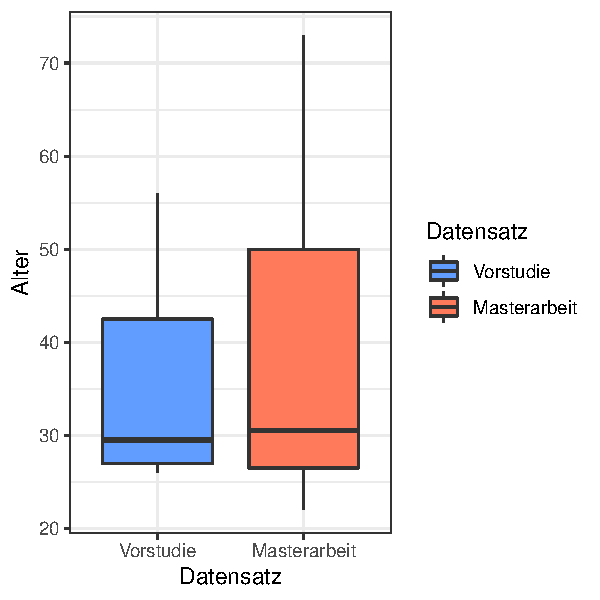
\includegraphics[width=1\columnwidth]{figures/boxplot.pdf}
    \caption{\label{fig:age-boxplot}Boxplot zur Altersverteilung von Testpersonen}
\end{figure}

% Alter
\autoref{fig:age-boxplot} zeigt die Altersverteilung der Testpersonen im Vergleich zur Vorstudie.
Dabei ist zu erkennen, dass die Altersverteilung der Masterarbeit eine höhere Anzahl an älteren Personen aufweist.
Auch die gesamte Altersverteilung der Masterarbeit weist eine breitere Streuung auf.
Speziell das höchste Alter von 73 Jahren ist damit wesentlich höher als das Maximalalter von 56 Jahren in der Vorstudie.
Jedoch liegt der Median der Masterarbeit (30.5) bei einem ähnlichen Wert wie in der Vorstudie (29.5).
Die beiden Testpersonen in der Altersklasse von 70 Jahren wurden als elementar für das Experiment angesehen.
Das liegt daran, dass die beiden Testpersonen einer älteren Generation angehören und eine weitere Zielgruppe für die Entwicklung des Prototyps darstellen.
Ebenfalls wurde sichergestellt, dass beide Testpersonen über eine ausreichende, aber keine hohe, technische Affinität verfügen.
Der Vorteil dieser Auswahl ist, dass bei diesen Testpersonen andere technische Probleme bei der Durchführung des Experiments als bei jüngeren Testpersonen auftreten können.\\

\begin{figure}[!ht]
    \centering
    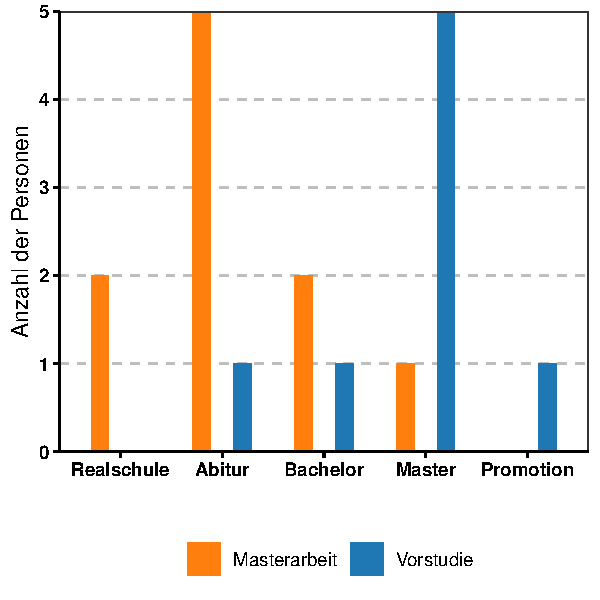
\includegraphics[width=0.7\columnwidth]{figures/education.pdf}
    \caption{\label{fig:education}Bildungsabschlüsse der Testpersonen}
\end{figure}

% Bildung
Bei den Bildungsabschlüssen der Testpersonen wurde ebenfalls darauf geachtet, dass diese die Bevölkerung in Deutschland besser abbilden als in der Vorstudie.
Die Bildungsabschlüsse Fachoberschule und Abitur wurden zusammengefasst.
Zusätzlich wurden die Bildungsabschlüsse Master und Diplom zusammengefasst.
\autoref{fig:education} zeigt deutlich, dass die Vorstudie eine hohe Anzahl an Personen mit Hochschulabschluss aufweist.
Dies spiegelt jedoch nicht die tatsächliche Verteilung der Bildungsabschlüsse in Deutschland wider \textcolor{red}{Abschlüsse DE}.
Auch wenn beide Datensätze nicht als repräsentativ angesehen werden können, spielt die Verteilung der Bildungsabschlüsse eine wichtige Rolle für die Entwicklung des Prototyps.
Das liegt daran, dass Bildungsabschlüsse oft mit verschiedenen Fähigkeiten einhergehen, welche bei der Entwicklung des Prototyps berücksichtigt werden müssen.
